%! TEX root = **/010-main.tex
% vim: spell spelllang=en:
\documentclass[aspectratio=169]{beamer}
\usetheme{metropolis}           % Use metropolis theme


\setbeamercolor{background canvas}{bg=white}

\usepackage{graphicx}
\graphicspath{{../figures/}}

\hypersetup{
    colorlinks,
   linkcolor={black},
   citecolor={black},
   %linkcolor={red!50!black},
   %citecolor={blue!50!black},
   urlcolor={blue!80!black}
}

\usepackage{booktabs}

\newcommand{\sresults}[2]{
\begin{table}[H]
\centering
\begin{tabular}{lc}
Confusion matrix on test set: & \( \begin{bmatrix} #1 \end{bmatrix} \) \\
    \addlinespace[0.5em]
    Accuracy on test set: & #2
\end{tabular}
\end{table}
}

\newcommand{\fresults}[3]{
\begin{table}[H]
\centering
\begin{tabular}{lc}
Confusion matrix on test set: & \( \begin{bmatrix} #1 \end{bmatrix} \) \\
    \addlinespace[0.5em]
    Accuracy on test set: & #2 \\
    F1 score on test set: & #3
\end{tabular}
\end{table}
}

\newcommand{\results}[7]{
\begin{table}[H]
\centering
\begin{tabular}{lc}
\toprule
\multicolumn{2}{c}{Best results (#4)} \\
\midrule
Confusion matrix on test set: & \( \begin{bmatrix} #1 \end{bmatrix} \) \\
    \addlinespace[0.5em]
    Accuracy on test set: & #2 \\
    F1 on test set: & #3 \\
    \addlinespace[1em]
    Number of supports: & #5 (#6 of them have slacks) \\
    Proportion of supports: & #7 \\
    \bottomrule
\end{tabular}
\end{table}
}

\title{NASA Kepler Exoplanet Search}
\subtitle{Data Mining}
\date{\today}
\author{
Aleix Boné \and
Eduard Bosch \and
David Gili \and
Albert Mercadé
}
\institute{UPC}

\begin{document}
  \maketitle
  
\section{Data source}
\begin{frame}{Our Dataset}
\begin{center}
    NASA's Exoplanet Search Results \footnote[frame]{Dataset URL: \url{https://www.kaggle.com/nasa/kepler-exoplanet-search-results}}
\vspace{5 mm}

\begin{columns}[t]
    \column{0.3\textwidth}
    
    \large
    \textbf{Original Dataset}
    
    \small
    
    9.564 data records
    
    8.48\% of missing data
    
    50 variables
    
    \column{0.3\textwidth}
    \large
    \textbf{Target column}
    
    \footnotesize
    \texttt{koi\_disposition}
    
    \begin{itemize}
        \itemsep0.05em
        \item[--] CONFIRMED
        \item[--] FALSE POSITIVE
        \item[--] (CANDIDATE)
        \item[--] (NOT DISPOSED)
    \end{itemize}
    % TODO
   
\end{columns}

\end{center}
\end{frame}


\begin{frame}{Goal}
\begin{quote}
The focus of the project is to correctly classify potential exoplanets based
on the raw measurements taken by NASA's Kepler Space Observatory.
\end{quote}
\end{frame}  

\section{Pre-processing}
\begin{frame}{Pre-processing steps}
\large
\begin{itemize}
     \itemsep0.5em
     \item Feature removal
     \item Example removal 
     \item Value transformation
     \item Error and missing data treatment
     \item Feature selection
\end{itemize}
\normalsize
\end{frame}

\begin{frame}{Feature selection}
    \vspace{0.75cm}
    \begin{figure}[H]
        \centering
        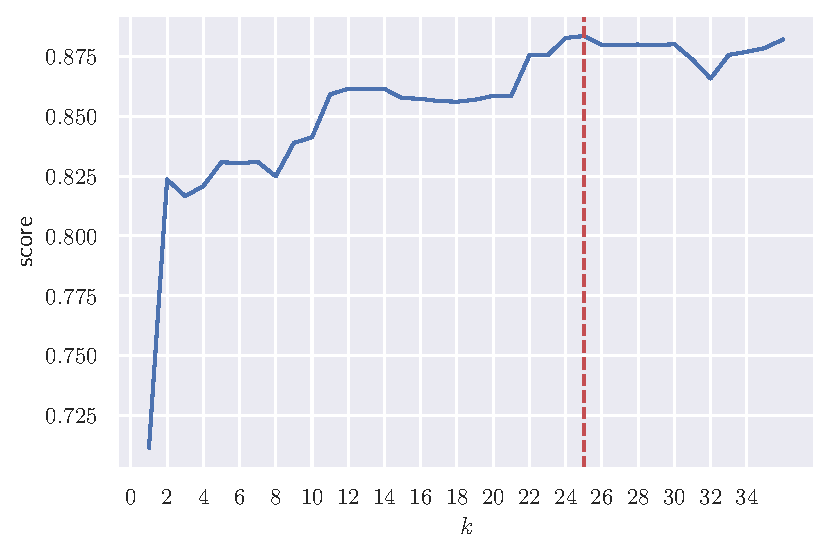
\includegraphics[width=0.5\linewidth]{kbest}
        \caption{Cross validation score for different $k$ values}%
        \label{fig:feature_cross}
    \end{figure}
\end{frame}

\begin{frame}{Evaluation criteria}
    \textbf{Validation Dataset}
    \small
    \begin{itemize}
    	\item[--] 30(test) : 70(training) split
    	\item[--] Target category proportions maintained
    \end{itemize}
    \normalsize
 
    \textbf{Parameter Optimization}
    
    \small
    5-fold cross validation
    
    \normalsize
    \textbf{Metrics}
    
    \small
    F-measure
    \normalsize
\end{frame}

\section{Execution of Machine Learning methods}

\begin{frame}{Na\"ive Bayes - Normalization}
\begin{table}[H]
\centering
\begin{tabular}{lccc}
\toprule
    & No normalization & Standardization & Power Transform \\
    \midrule
    Confusion matrix & 
    \( \begin{bmatrix} 208 & 200 \\ 3 & 189 \end{bmatrix} \) & 
    \( \begin{bmatrix} 287 & 121 \\ 2 & 190\end{bmatrix} \) &
    \( \begin{bmatrix} 357 & 51 \\ 19 & 173\end{bmatrix} \)
    \\
    \addlinespace[0.5em]
    Accuracy: & 0.661 & 0.795 & 0.883 \\
    F1 score: & 0.65 & 0.755 & 0.831 \\
    \bottomrule
\end{tabular}
\end{table}
\end{frame}

\begin{frame}{Na\"ive Bayes - Parameter tuning}
\begin{figure}[H]
    \centering
    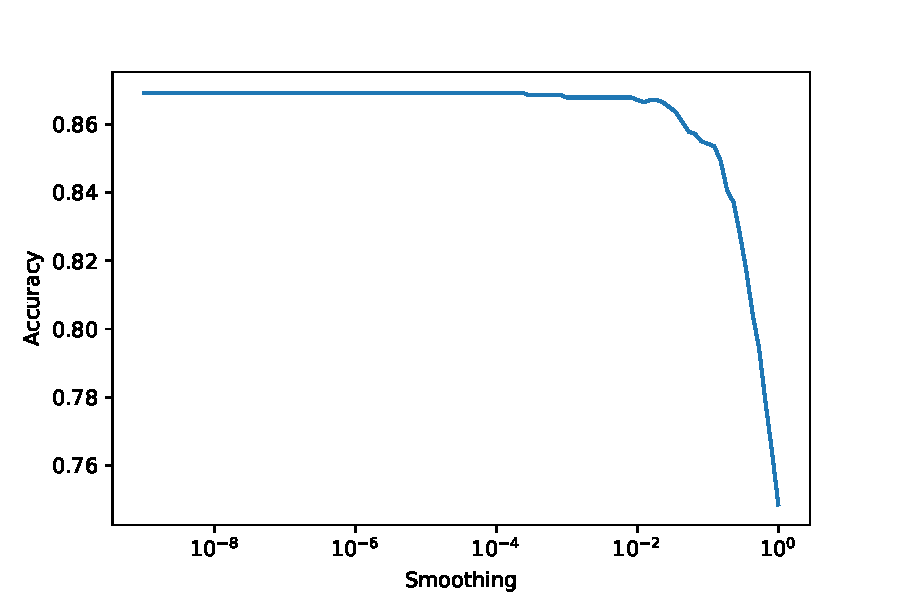
\includegraphics[width=0.6\textwidth]{naive_bayes_smoothing_cv.pdf}
    \caption{Na\"ive Bayes smoothing}%
    \label{fig:naive_bayes_smoothing_cv}
\end{figure}
\end{frame}

\begin{frame}{K-NN}
\begin{figure}[H]
    \centering
    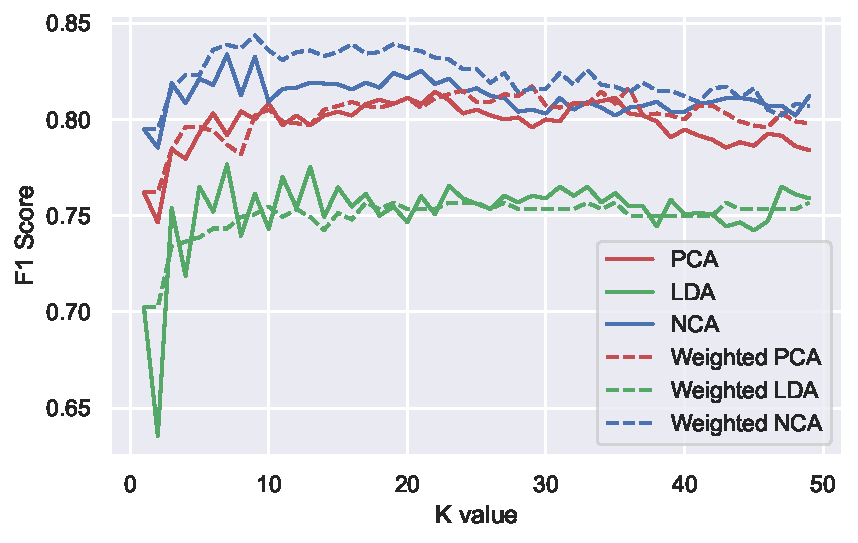
\includegraphics[width=0.6\textwidth]{knn}
    \caption{weighted and unweighted knn with PCA, LDA and NCA}%
    \label{fig:knn_pca_lda_nca}
\end{figure}
\end{frame}

\begin{frame}{K-NN}

\fresults{ 367 &  41 \\ 22 & 170 }{0.895}{0.844}

\end{frame}

\begin{frame}{Decision Trees - Parameter tuning}
\begin{figure}[H]
    \centering
    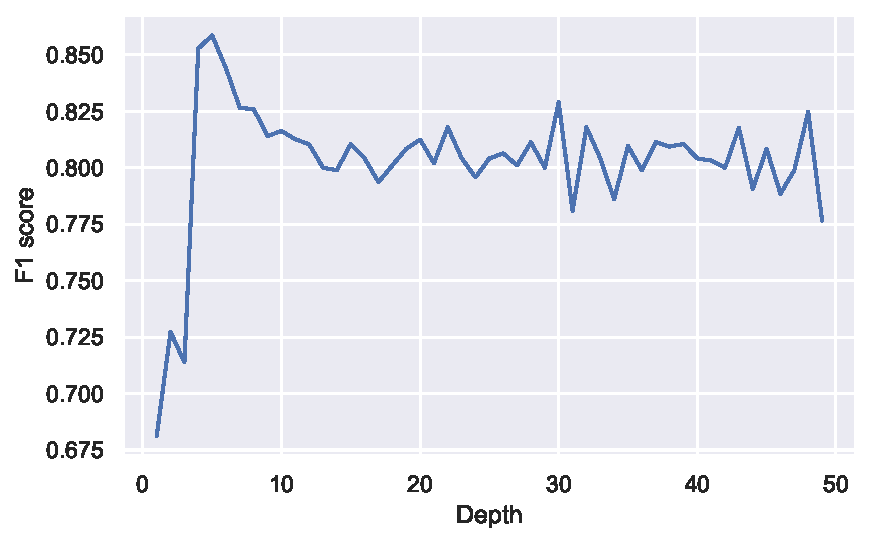
\includegraphics[width=0.6\textwidth]{decision_trees}
    \caption{Decision trees F1 Score depending on the maximum depth of the decision tree.}%
    \label{fig:decision_trees_acc}
\end{figure}
\end{frame}

\begin{frame}{Decision Trees}
\begin{figure}[H]
    \centering
    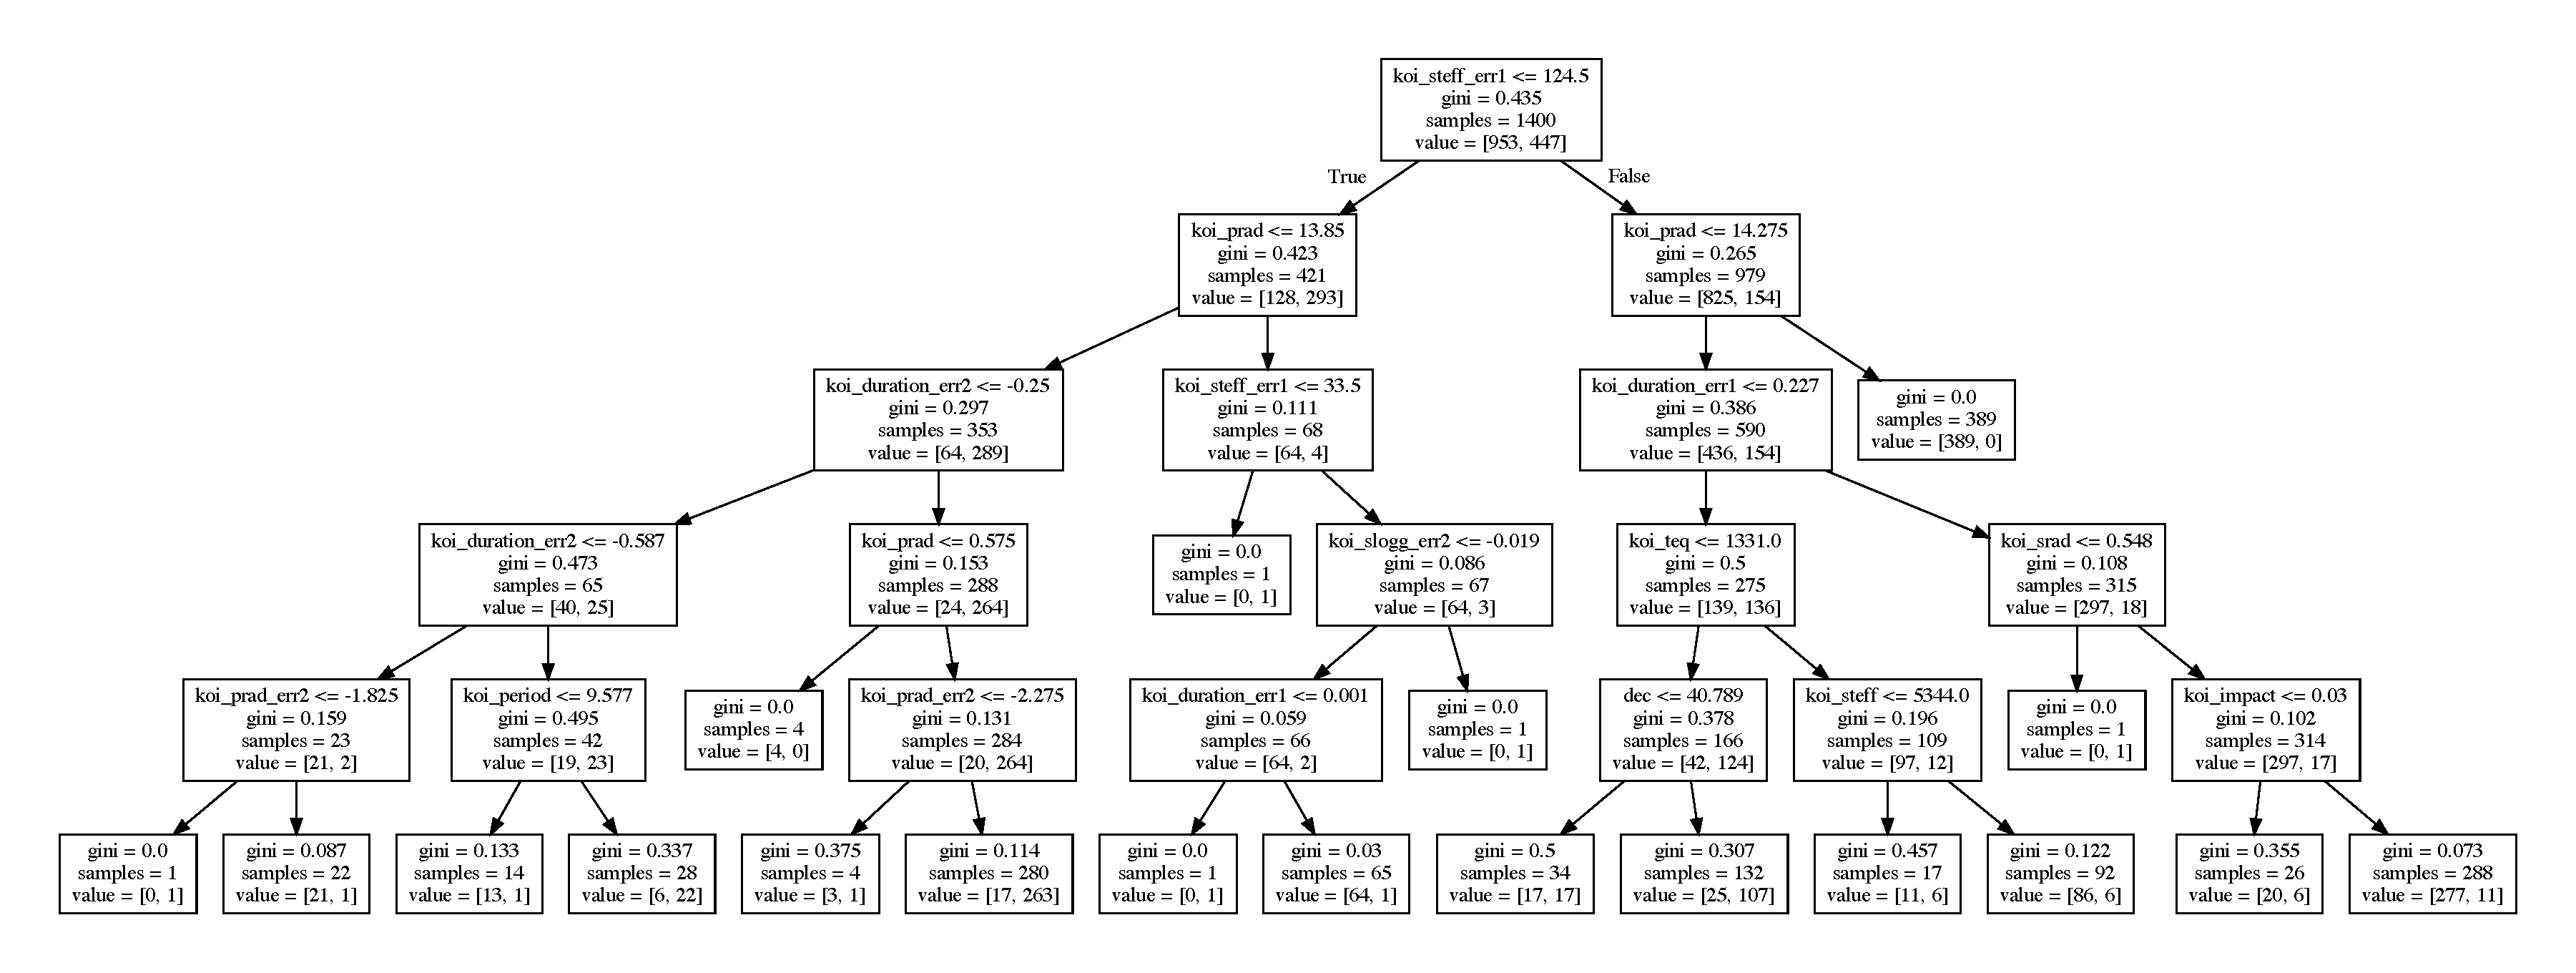
\includegraphics[width=\textwidth]{decision_tree}
    \caption{Our best-performing decision tree.}%
    \label{fig:decision_trees}
\end{figure}
\end{frame}

\begin{frame}{Support Vector Machines - Lineal kernel}

\begin{figure}[H]
    \centering
    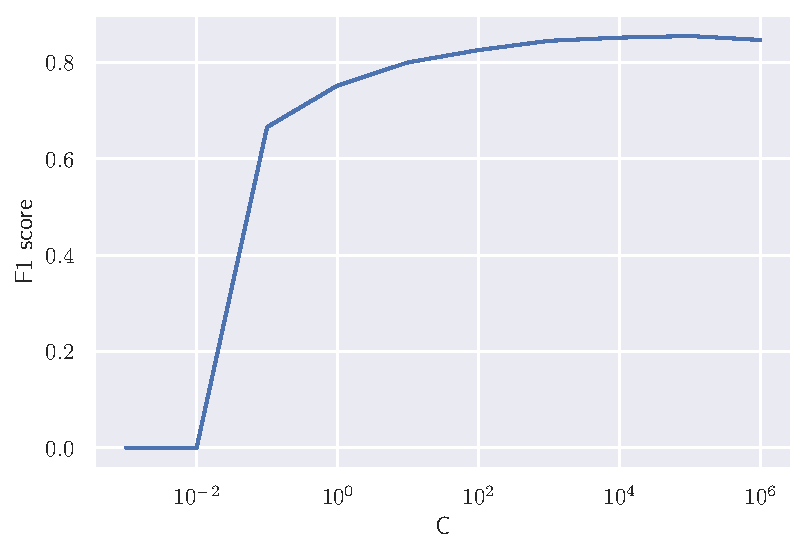
\includegraphics[width=0.6\textwidth]{svm_linear_C_cv}
    \caption{linear SVM C parameter search}%
    \label{fig:svm_linear_C_cv}
\end{figure}

\end{frame}

\begin{frame}{Support Vector Machines - Lineal kernel}
\results{383 & 25 \\ 26 & 166}{0.915}{0.8668}{$C=10^5$}{288}{269}{0.2057}
\end{frame}

\begin{frame}{Support Vector Machines - Polynomial and RBF kernels}
\begin{table}[H]
\caption{Comparison of different SVM kernels}
\begin{tabular}{lcccccc}
\toprule
Kernel       & Accuracy & F1 & Supports & Proportion & C & $\gamma$ \\
\midrule
Linear       & 0.9150 & 0.8668 & 288(269) & 0.2057 & $10^5$\\
Polynomial 2 & 0.9067 & 0.8542 & 332(283) & 0.2371 & $10^4$\\
Polynomial 3 & 0.9050 & 0.8503 & 356(317) & 0.2543 & $10^3$\\
RBF          & 0.9083 & 0.8564 & 330(302) & 0.2357 & $10^6$ & 0.001\\
\bottomrule
\end{tabular}
\end{table}

\end{frame}

\subsection{Meta-learning algorithms}

\begin{frame}[allowframebreaks]{Performance majority voting}
\begin{table}[H]
\centering
\caption{Majority voting results}
\begin{tabular}{lr}
\toprule
Method & Accuracy \\
\midrule
Na\"ive Bayes & 0.884 \\
K-NN & 0.857 \\
Decision Tree & 0.877 \\
\addlinespace[0.5em]
Majority voting & 0.914 \\
Majority voting (weighted)  & 0.914 \\
\bottomrule
\end{tabular}
\end{table}

\framebreak

With hard voting:
\sresults{ 375 &  33 \\ 20 & 172 }{ 0.9117 }

\noindent
With weighted voting (2 1 2):
\sresults{ 373 &  35 \\ 19 & 173 }{ 0.9100 }
\end{frame}

\begin{frame}{Bagging}
\begin{figure}[H]
\centering
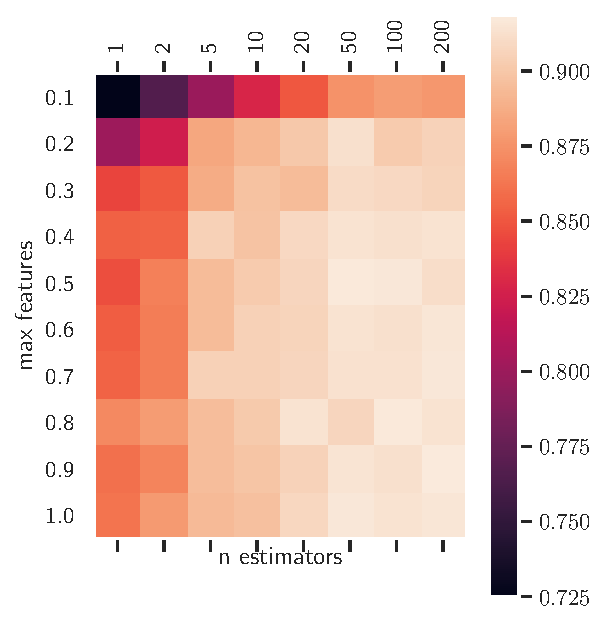
\includegraphics[width=0.4\textwidth]{bagging}
\caption{Bagging parameter search}%
\label{fig:bagging}
\end{figure}

\end{frame}
\begin{frame}{Bagging}

Best results:  $\texttt{n\_est} = 200,\, \texttt{max\_features} = 0.9$

\sresults{ 388 &  20 \\ 24  & 168 }{0.9267}
\end{frame}

\begin{frame}{Random Forest}
\begin{table}[H]
\centering
\caption{RandomForest best parameters}
\begin{tabular}{lr}
\toprule
Parameter & Value \\
\midrule
\texttt{bootstrap} & True \\
\texttt{max\_depth} & 150 \\
\texttt{max\_features} & 10 \\
\texttt{min\_samples\_leaf} & 5 \\
\texttt{min\_samples\_split} & 5 \\
\texttt{n\_estimators} & 500 \\
\bottomrule
\end{tabular}
\end{table}
\end{frame}

\begin{frame}{Adaboost}
\fresults{ 384 &  24 \\ 21 & 171 }{0.925}{0.883}
\end{frame}

\begin{frame}{AdaBoost}
\begin{figure}[H]
\centering
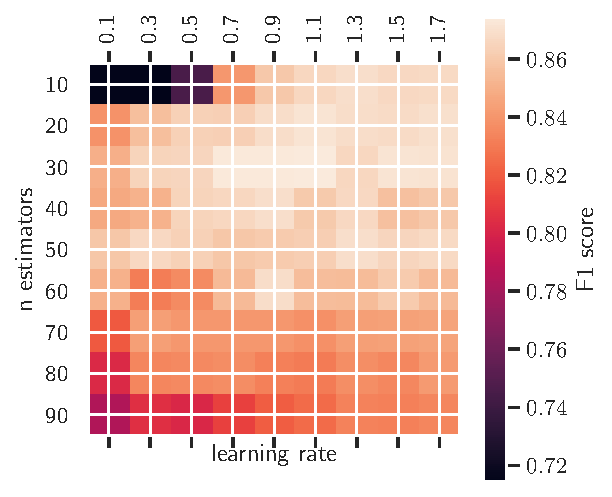
\includegraphics[width=0.5\textwidth]{boosting}
\caption{AdaBoost parameter search}%
\label{fig:boosting}
\end{figure}

\end{frame}
\begin{frame}{AdaBoost}
When executing Adaboost with the best parameters found we obtain the following results:

\fresults{ 383 &  25 \\ 21 & 171 }{0.923}{0.881}
\end{frame}

\section{Comparison}

\begin{frame}{Comparison - Accuracy and F1}
\begin{table}[H]
\centering
\caption{Comparison of metrics}%
\label{tab:comparison}
\begin{tabular}{lrr}
\toprule
{} &  Accuracy &        F1 \\
\midrule
nb     &  0.871667 &  0.813559 \\
knn    &  0.856667 &  0.788177 \\
dt     &  0.910000 &  0.858639 \\
svm    &  0.911667 &  0.865140 \\
voting &  0.908333 &  0.858612 \\
bag    &  0.925000 &  0.882507 \\
rf     &  0.925000 &  0.881890 \\
ada    &  0.923333 &  0.881443 \\
\bottomrule
\end{tabular}

\end{table}
\end{frame}

\begin{frame}{Comparison - mcNemar}
\begin{figure}[H]
\centering
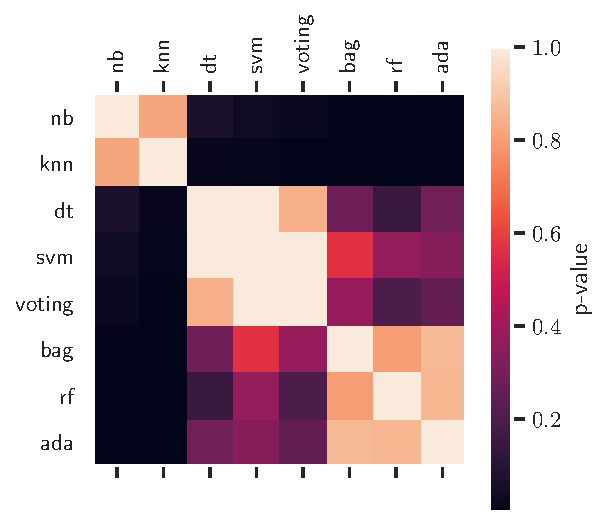
\includegraphics[width=0.6\textwidth]{chi_mcnemar_pvalue}
\caption{mcNemar test $p$-value}
\end{figure}
\end{frame}

\section{Thank you for your attention, any questions?}
\section{Thank you for your attention, any questions? I guess not :/}

\end{document}
